%% LaTeX-Beamer template for KIT design
%% by Erik Burger, Christian Hammer
%% title picture by Klaus Krogmann
%%
%% version 2.1
%%
%% mostly compatible to KIT corporate design v2.0
%% http://intranet.kit.edu/gestaltungsrichtlinien.php
%%
%% Problems, bugs and comments to
%% burger@kit.edu

\documentclass[18pt]{beamer}

%% SLIDE FORMAT

% use 'beamerthemekit' for standard 4:3 ratio
% for widescreen slides (16:9), use 'beamerthemekitwide'

\usepackage{./templates/beamerthemekit}
% \usepackage{templates/beamerthemekitwide}


\titleimage{kde-and-trajectories}



\title{Kernel Density Estimates and Mean Shift Clustering}
% \subtitle{Sommersemester 2018}
\author{Jonas Spinner}
\date{February 4, 2019}

\institute{Analytics and Statistics at the Institute of Operations Research}

% Bibliography

\usepackage{natbib}

%\usepackage[citestyle=authoryear,bibstyle=numeric,hyperref,backend=biber]{biblatex}
%\addbibresource{../latex/KDEaMSC.bib}
%\bibhang1em


%\usepackage{tikz}

%\usepackage{algorithm}
%\usepackage{algorithmic}

\usepackage{algpseudocode}
\usepackage{algorithm}
% keine "End"-Statements in Algorithmen
\algtext*{EndWhile}
\algtext*{EndIf}
\algtext*{EndFor}
\algtext*{EndProcedure}


\usepackage[utf8]{inputenc}
\usepackage[english]{babel}
\usepackage[T1]{fontenc}
\usepackage{amsmath,amsmath,lmodern}
\usepackage{bm}
\usepackage{bbm}

\usepackage{graphicx}
\usepackage{subfig}

\usepackage[font=scriptsize]{caption}



\newcommand{\norm}[1]{\left\lVert#1\right\rVert}



\begin{document}

% change the following line to "ngerman" for German style date and logos
% \selectlanguage{ngerman}

%title page
\begin{frame}
\titlepage
\end{frame}

%table of contents
\begin{frame}{Outline}
	\tableofcontents
\end{frame}


\section{Introduction}


\section{Kernel Density Estimates}

\begin{frame}{Density estimation}
	\begin{figure}
		\tiny
		\centering
		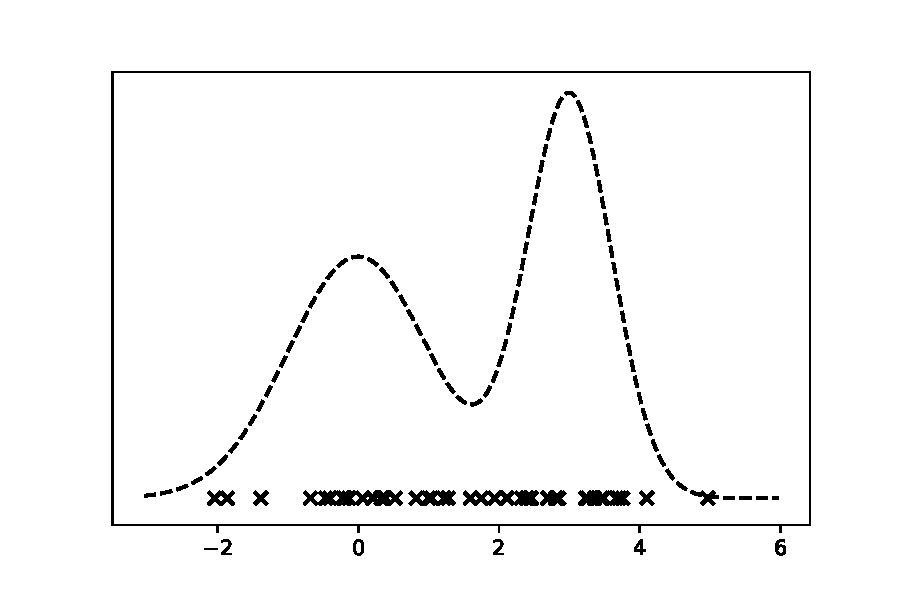
\includegraphics[height=0.5\textheight]{figures/samples-and-underlying-pdf}
		%\vspace*{-4mm}
		%\caption{Author's illustration.}
	\end{figure}
	\vspace*{-4mm}
	\begin{itemize}
		\item \textbf{Task}: Given samples $\bm{x}_1, ..., \bm{x}_n \in \mathbb{R}^d$, estimate the underlying density.
		%\item \textbf{Assumptions}: $\bm{x}_i$ are independent and identically distributed with probability density distribution $f(\bm{x})$.
	\end{itemize}
\end{frame}


\subsection{Definition}

\begin{frame}{The kernel density estimate}
	The kernel density estimate is defined as:
	\begin{align*}
		\hat{f}(\bm{x}) = \frac{1}{n h^d} \sum_{i=1}^{n} K\left(\frac{\bm{x} - \bm{x}_i}{h} \right)
	\end{align*}
	
	\begin{itemize}
		\item $K$ is a \textit{kernel function}.
		\item $h$ is a \textit{bandwidth parameter}.
	\end{itemize}
	\begin{itemize}
		\item When $\int_{\mathbb{R}^d} K(\bm{x}) dx = 1$ and $K(\bm{x}) \geq 0$ for all $\bm{x}$ then $\hat{f}(\bm{x})$ is a valid probability density function.
	\end{itemize}
\end{frame}


\subsection{Kernel functions}


\begin{frame}{Popular kernel functions}
	\textbf{Radially symmetric kernel functions} are kernel functions which can be represented as
	
	\begin{align*}
		K(\bm{x}) = c_{k,d}\ k\left(\norm{\bm{x}}^2\right)
	\end{align*}
	
	\begin{itemize}
		\item $k(u) : [0, \infty) \rightarrow [0, \infty)$ is called the profile of $K$.
		\item For example the gaussian kernel has the profile $k(u) = \exp(-\frac{1}{2}u)$.
		\item Nearly all popular kernel belong to this class of kernels.
	\end{itemize}
\end{frame}


\begin{frame}{Popular kernel functions}
	\centering
	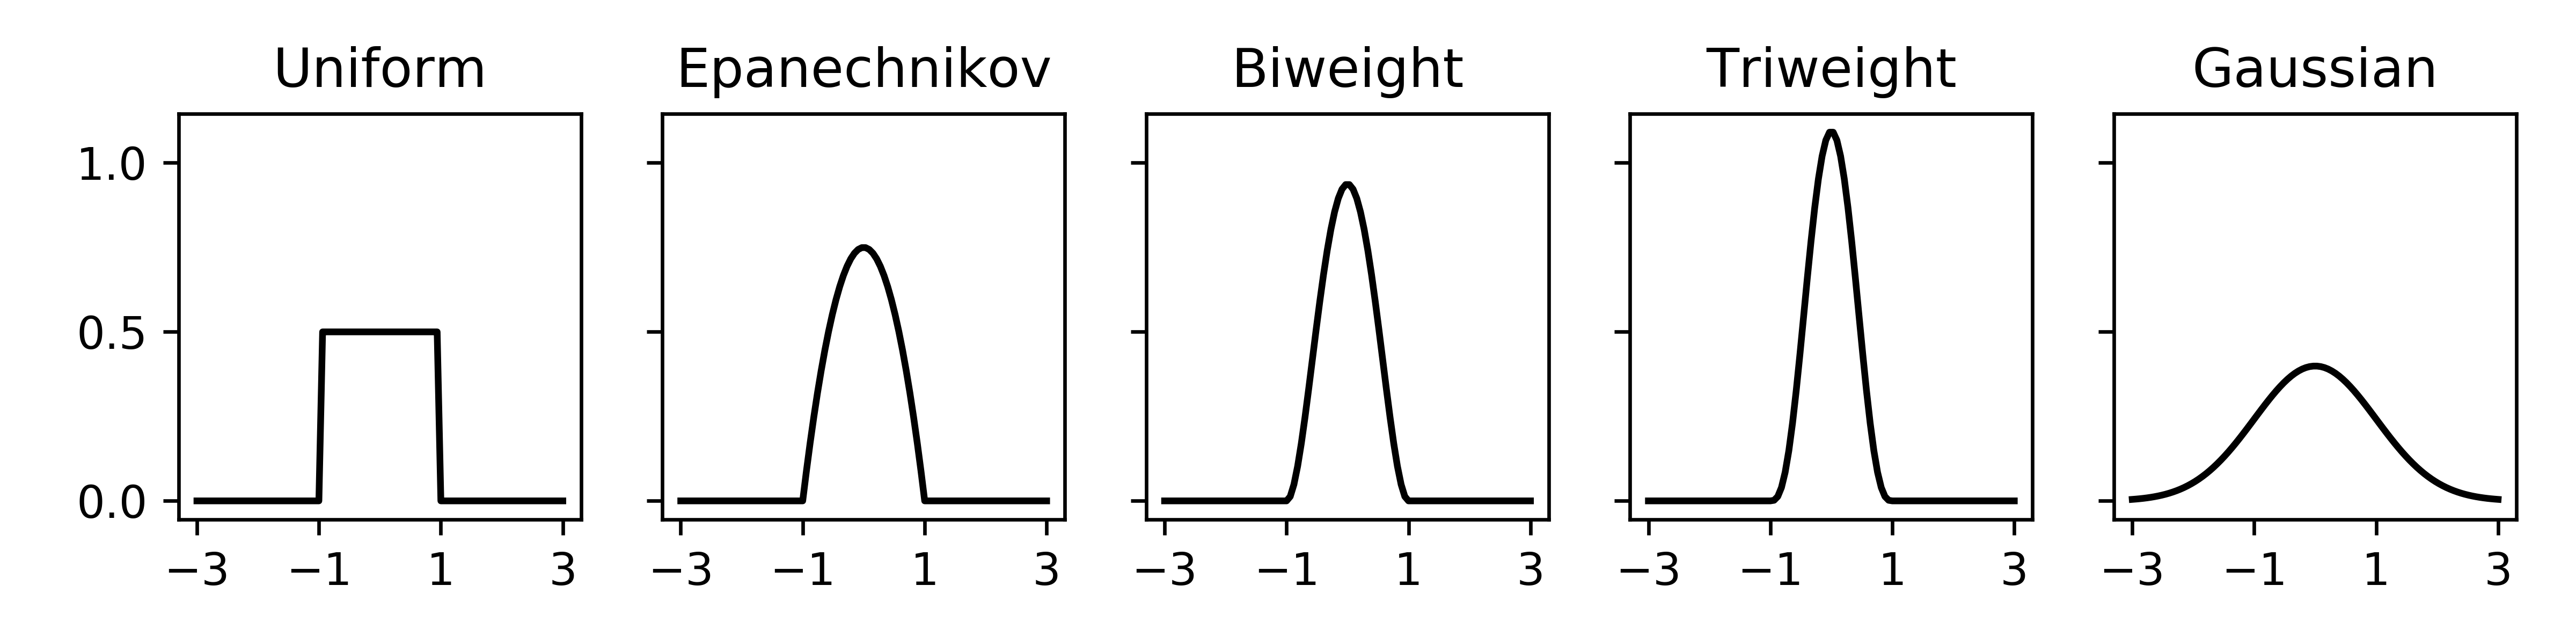
\includegraphics[width=0.9\textwidth]{figures/kde-popular-kernels}
	\begin{table}
		\begin{center}
			\tiny
			\begin{tabular}{r|r|r|r|l}
				\textbf{Name} & \textbf{Profile support} & $k(u)$ & $-k'(u)$ & $K(\bm{x})$ \\ \hline\hline
				Uniform & $u \in [0, 1]$ & $1$ & $0$ & $\text{vol}\left(S_d\right)^{-1}$ \\
				Epanechnikov & $u \in [0, 1]$ & $1 - u$ & $1$ & $\frac{1}{2} \text{vol}(S_d)^{-1} (d+2) \left(1 - \norm{\bm{x}}^2\right)$\\
				Biweight & $u \in [0, 1]$ & $(1 - u)^2$ & $2 (1 - u)$ & $\propto \left(1 - \norm{\bm{x}}^2\right)^2$ \\
				Triweight & $u \in [0, 1]$ & $(1 - u)^3$ & $3 (1 - u)^2$ & $\propto \left(1 - \norm{\bm{x}}^2\right)^3$ \\
				Gaussian & $u \in [0, \infty)$ & $\exp\left(-\frac{1}{2}u\right)$ & $\frac{1}{2}\exp\left(-\frac{1}{2}u\right)$ & $(2\pi)^{-d/2} \exp\left(-\frac{1}{2}\norm{\bm{x}}^2\right)$
			\end{tabular}
		\end{center}
	\end{table}
\end{frame}

\begin{frame}{Bandwidth}
	\begin{figure}
		\includegraphics<1>[width=\textwidth]{figures/kernel-density-estimation-gaussian-50}
		\includegraphics<2>[width=\textwidth]{figures/kernel-density-estimation-uniform-50}
		\includegraphics<3>[width=\textwidth]{figures/kernel-density-estimation-epanechnikov-50}
		\vspace*{-6mm}
		\caption{\only<1>{Gaussian kernel}\only<2>{Uniform kernel}\only<3>{Epanechnikov kernel}, $n = 50$.}
	\end{figure}
	\begin{itemize}
		\item The choice of bandwidth is a bias-variance tradeoff for the estimate $\hat{f}(\bm{x})$.
		\item A small bandwidth results in high variance, a large bandwidth introduces a bias.
	\end{itemize}
\end{frame}



\section{Mean Shift Clustering}


\begin{frame}{History}
\begin{itemize}
	\item Introduced by \cite{Fukunaga.1975}
	\item Popularized for computer vision tasks \cite{Comaniciu.2002} and \cite{Comaniciu.2003}. Image segmentation, image filtering and object tracking
\end{itemize}
\end{frame}


\begin{frame}{Locally weighted mean}
	The weighted mean
	\begin{align*}
		\bm{\mu}^* = \frac{\sum_{i=1}^n \bm{x}_i w_i}{\sum_{i=1}^n w_i}
	\end{align*}
	
	The locally weighted mean has weights depending on the distance to a data point $\bm{x}$
	\begin{align*}
		\bm{\mu}^*(\bm{x}) = \frac{\sum_{i=1}^n \bm{x}_i\ g\left(\norm{\frac{\bm{x} - \bm{x}_i}{h}}^2 \right)}{\sum_{i=1}^n g\left(\norm{\frac{\bm{x} - \bm{x}_i}{h}}^2 \right)}
	\end{align*}
\end{frame}


\begin{frame}
	\begin{align*}
		\bm{x}^{(t+1)} &= \frac{\sum_{i=1}^n \bm{x}_i\ g\left(\norm{(\bm{x}^{(t)} - \bm{x}_i) / h}^2 \right)}{\sum_{i=1}^n g\left(\norm{(\bm{x}^{(t)} - \bm{x}_i) / h}^2 \right)} & \text{for } i = 1, 2, ... \\[1em]
		&= \bm{x}^{(t)} + \bm{m}\left(\bm{x}^{(t)}\right) &
	\end{align*}
\end{frame}

\begin{frame}{Connecting the mean shift vector and kernel density estimation}
	\begin{itemize}
		\item \textbf{Result}: the mean shift vector $\bm{m}(\bm{x})$ points into the gradient direction of a kernel density estimate. 
	\end{itemize}
	\begin{align*}
		\bm{m}(\bm{x}) = \bm{\mu}^*(\bm{x}) - \bm{x} = \frac{h^2c_{g,d}}{2c_{k,d}} \frac{\nabla \hat{f}_{h,K}(\bm{x})}{\hat{f}_{h,G}(\bm{x})}
	\end{align*}
\end{frame}


\subsection{Convergence}

\begin{frame}{Convergence -- Gaussian kernel}
	\includegraphics<1>[width=\textwidth]{figures/iterations-gaussian/step-1}
%	\includegraphics<2>[width=\textwidth]{figures/iterations-gaussian/step-2}
%	\includegraphics<3>[width=\textwidth]{figures/iterations-gaussian/step-3}
%	\includegraphics<4>[width=\textwidth]{figures/iterations-gaussian/step-4}
%	\includegraphics<5>[width=\textwidth]{figures/iterations-gaussian/step-5}
%	\includegraphics<6>[width=\textwidth]{figures/iterations-gaussian/step-6}
%	\includegraphics<7>[width=\textwidth]{figures/iterations-gaussian/step-7}
%	\includegraphics<8>[width=\textwidth]{figures/iterations-gaussian/step-8}
%	\includegraphics<9>[width=\textwidth]{figures/iterations-gaussian/step-9}
%	\includegraphics<10>[width=\textwidth]{figures/iterations-gaussian/step-10}
%	\includegraphics<11>[width=\textwidth]{figures/iterations-gaussian/step-11}
%	\includegraphics<12>[width=\textwidth]{figures/iterations-gaussian/step-12}
%	\includegraphics<13>[width=\textwidth]{figures/iterations-gaussian/step-13}
%	\includegraphics<14>[width=\textwidth]{figures/iterations-gaussian/step-14}
%	\includegraphics<15>[width=\textwidth]{figures/iterations-gaussian/step-15}
%	\includegraphics<16>[width=\textwidth]{figures/iterations-gaussian/step-16}
%	\includegraphics<17>[width=\textwidth]{figures/iterations-gaussian/step-17}
\end{frame}

\begin{frame}{Convergence -- Uniform kernel}
	\includegraphics<1>[width=\textwidth]{figures/iterations-uniform/step-1}
%	\includegraphics<2>[width=\textwidth]{figures/iterations-uniform/step-2}
%	\includegraphics<3>[width=\textwidth]{figures/iterations-uniform/step-3}
%	\includegraphics<4>[width=\textwidth]{figures/iterations-uniform/step-4}
%	\includegraphics<5>[width=\textwidth]{figures/iterations-uniform/step-5}
%	\includegraphics<6>[width=\textwidth]{figures/iterations-uniform/step-6}
%	\includegraphics<7>[width=\textwidth]{figures/iterations-uniform/step-7}
%	\includegraphics<8>[width=\textwidth]{figures/iterations-uniform/step-8}
%	\includegraphics<9>[width=\textwidth]{figures/iterations-uniform/step-9}
%	\includegraphics<10>[width=\textwidth]{figures/iterations-uniform/step-10}
%	\includegraphics<11>[width=\textwidth]{figures/iterations-uniform/step-11}
%	\includegraphics<12>[width=\textwidth]{figures/iterations-uniform/step-12}
%	\includegraphics<13>[width=\textwidth]{figures/iterations-uniform/step-13}
\end{frame}


\subsection{Bandwidth effects}

\begin{frame}{Bandwidth effects}
	\begin{itemize}
		\item The choice of bandwidth influences the density estimation and therefore the clustering outcome
	\end{itemize}
	\begin{itemize}
		\item Small bandwidth $\Rightarrow$ many density peaks / clusters
		\item Large bandwidth $\Rightarrow$ few peaks / clusters
	\end{itemize}
\end{frame}
\begin{frame}{Small bandwidth}
\begin{figure}
	\tiny
	\begin{tabular}{c}
		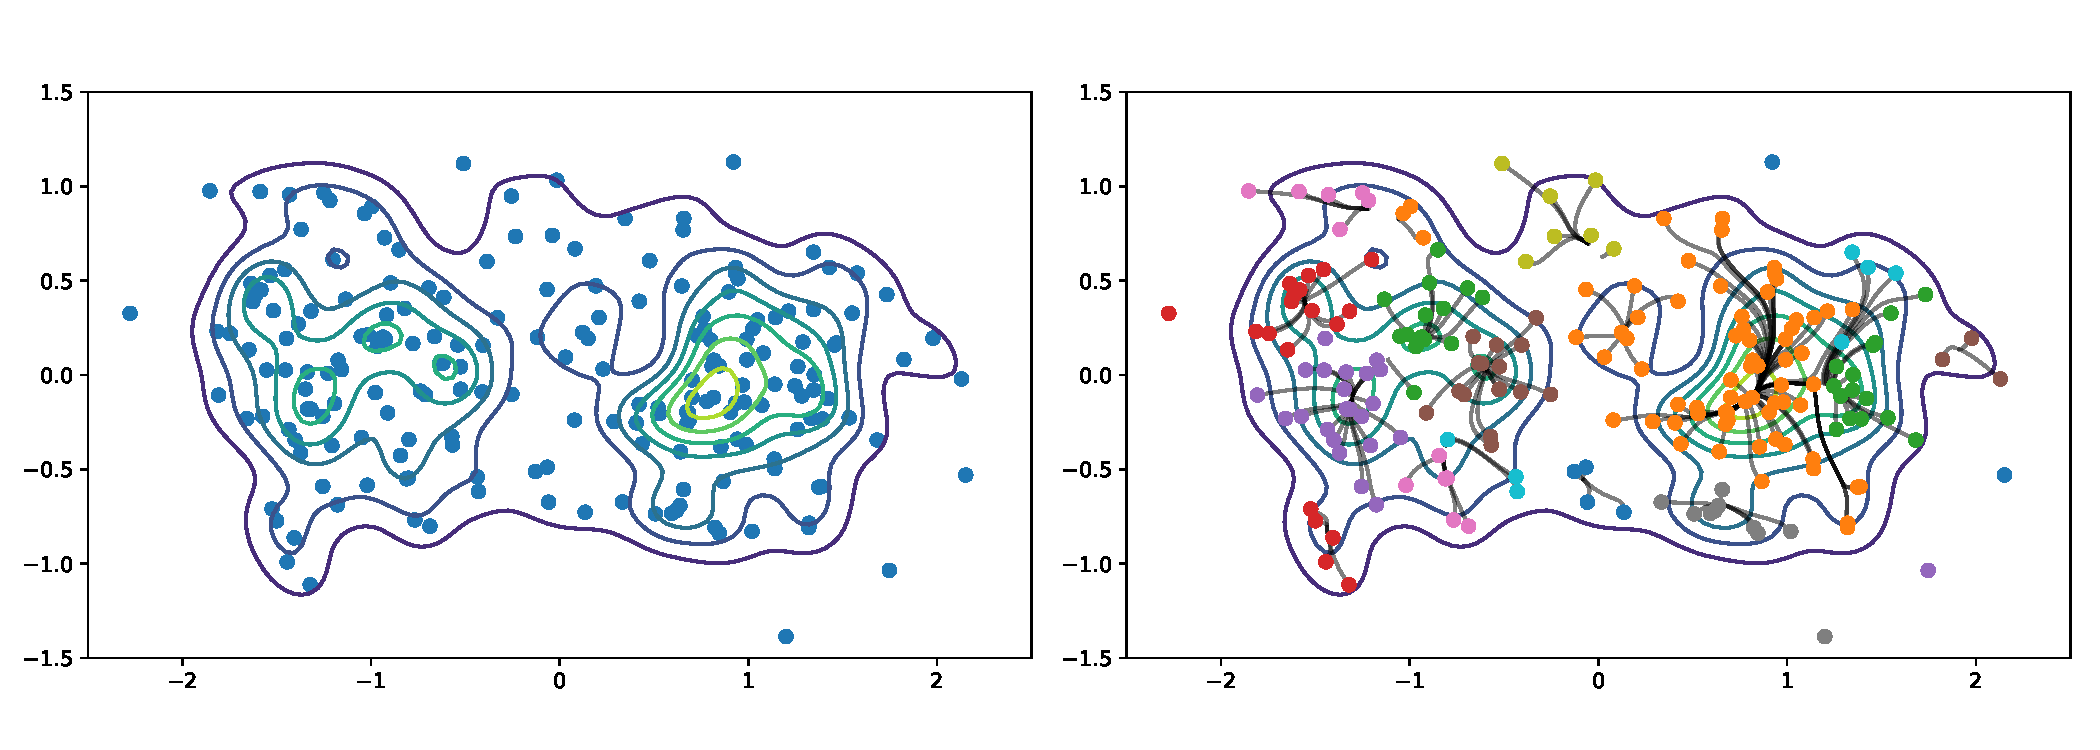
\includegraphics[height=0.4\textheight]{{{figures/contour/kde-and-trajectories-h=0.15-K=gaussian}}} \\[-2mm]
		$h=0.15$, gaussian kernel \\
		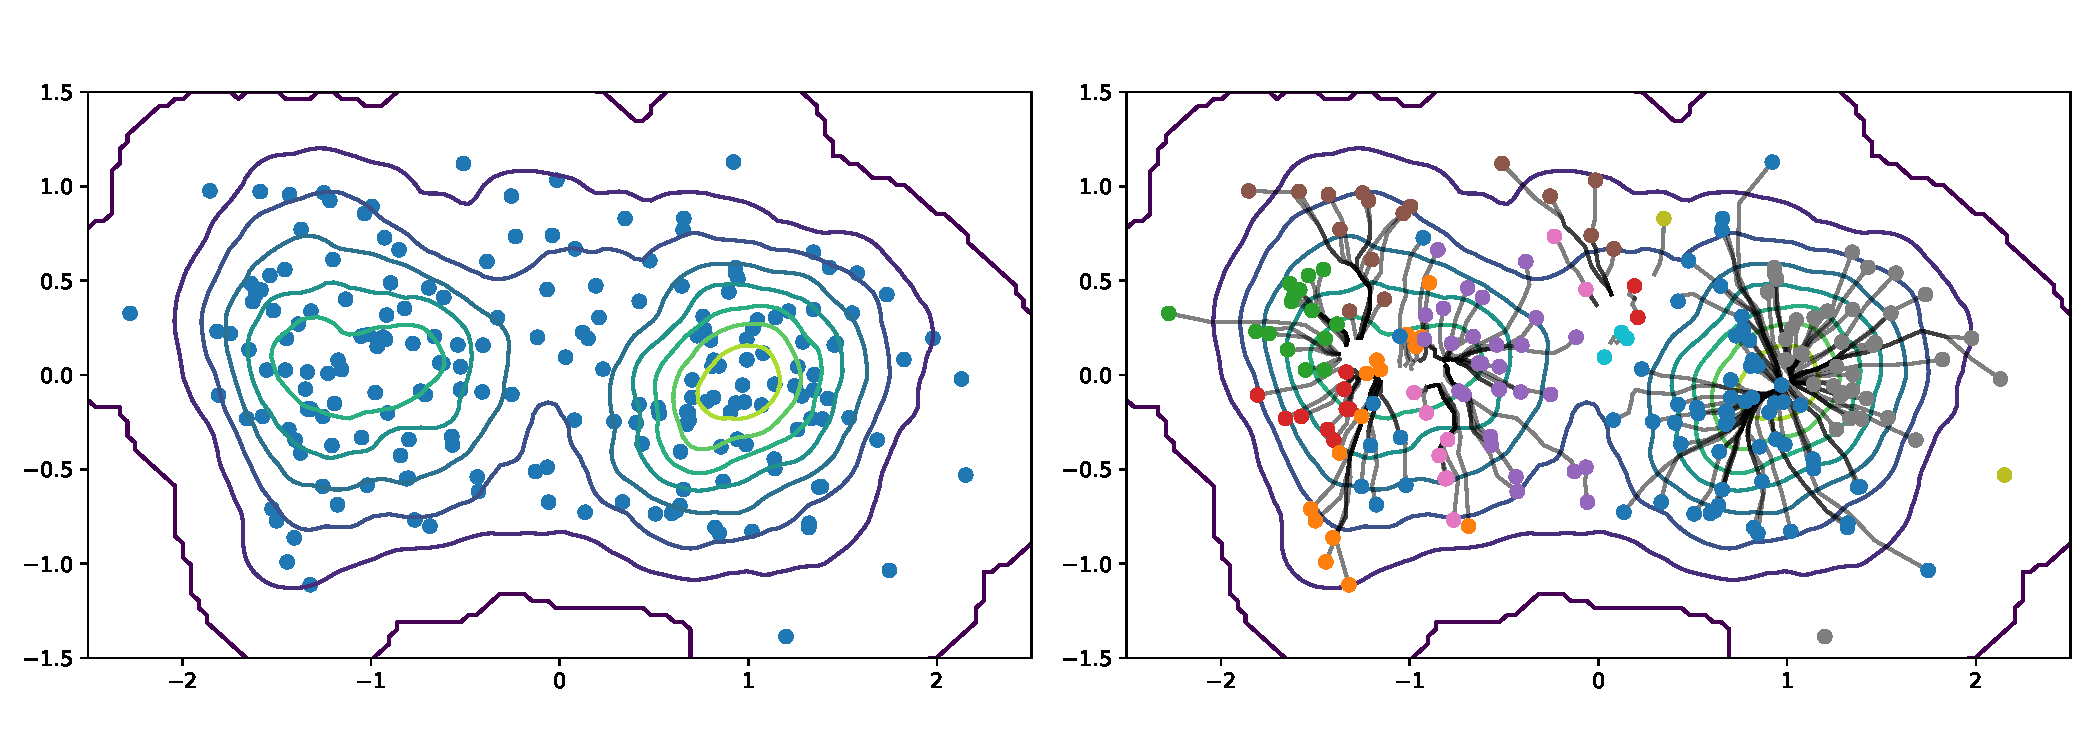
\includegraphics[height=0.4\textheight]{{{figures/contour/kde-and-trajectories-h=0.5-K=uniform}}} \\[-2mm]
		$h=0.5$, uniform kernel
	\end{tabular}
\end{figure}
\end{frame}

\begin{frame}{Middle bandwidth}
\begin{figure}	
	\tiny
	\begin{tabular}{c}
		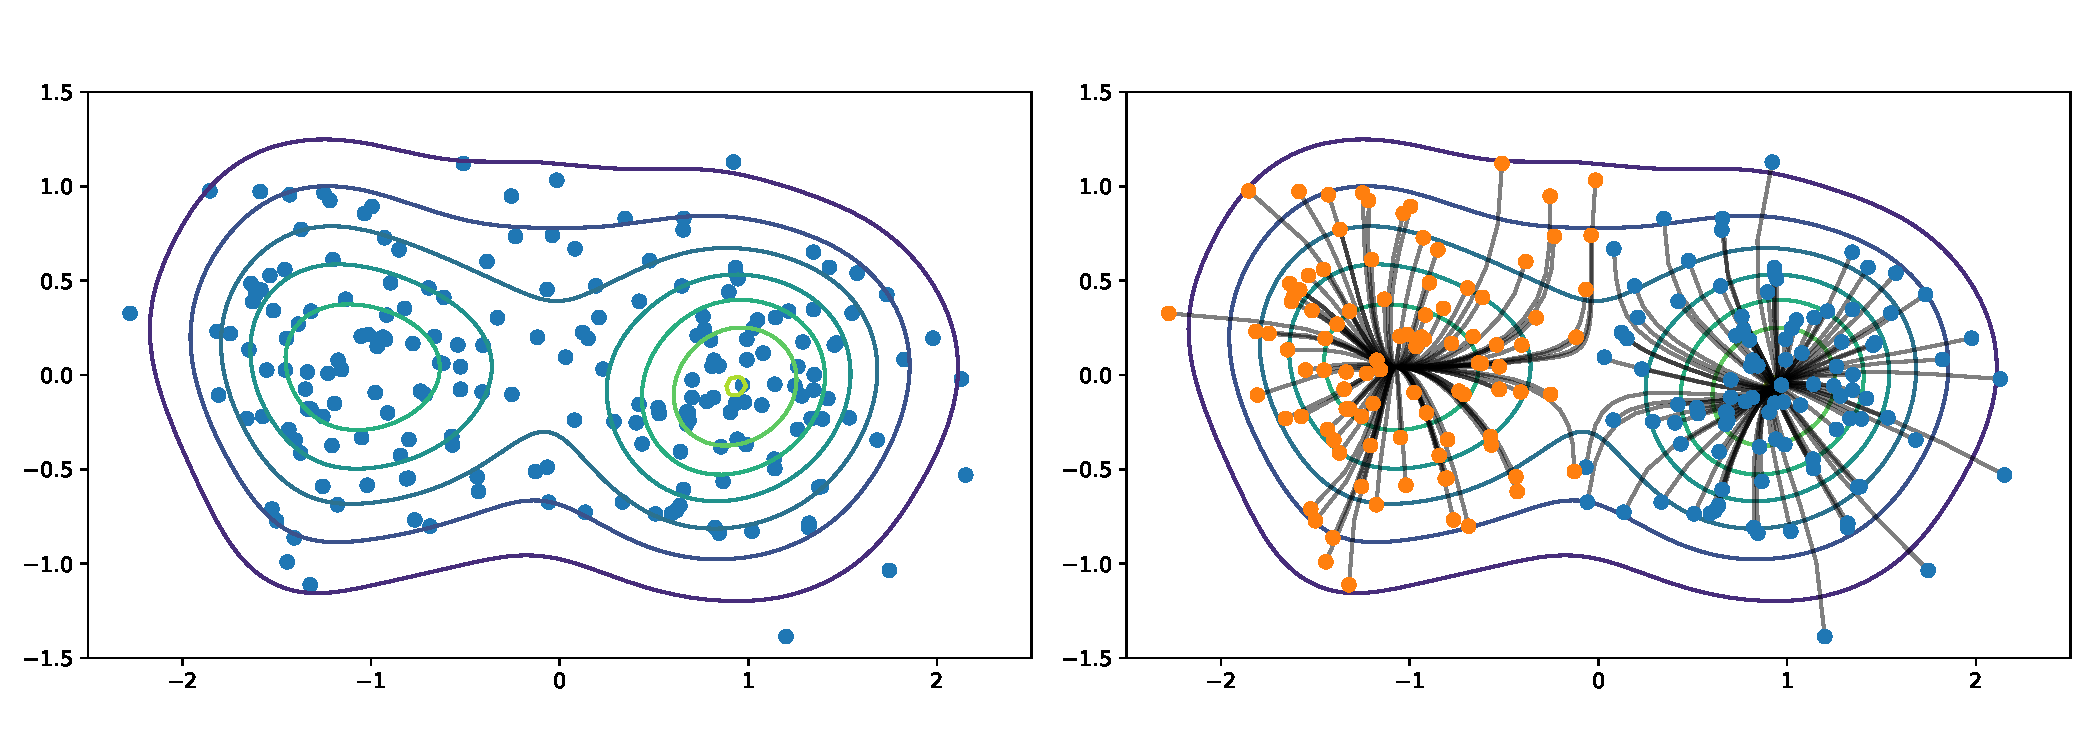
\includegraphics[height=0.4\textheight]{{{figures/contour/kde-and-trajectories-h=0.35-K=gaussian}}} \\[-2mm]
		$h=0.35$, gaussian kernel \\
		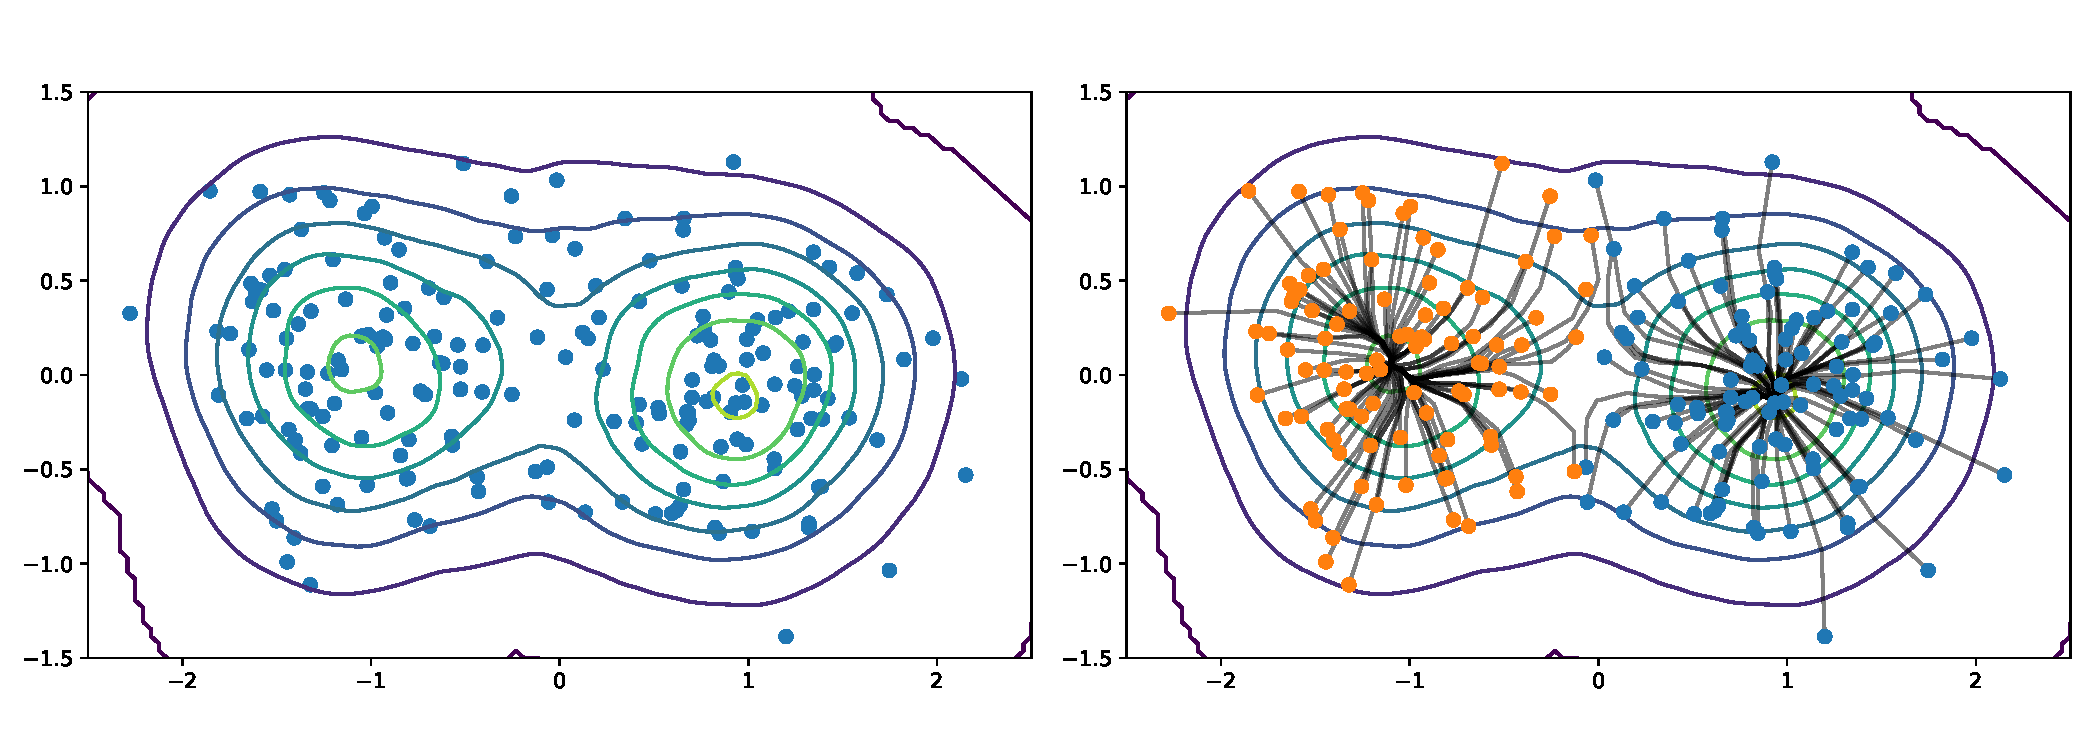
\includegraphics[height=0.4\textheight]{{{figures/contour/kde-and-trajectories-h=0.8-K=uniform}}} \\[-2mm]
		$h=0.8$, uniform kernel
	\end{tabular}
\end{figure}
\end{frame}

\begin{frame}{Large bandwidth}
\begin{figure}	
	\tiny
	\begin{tabular}{c}
		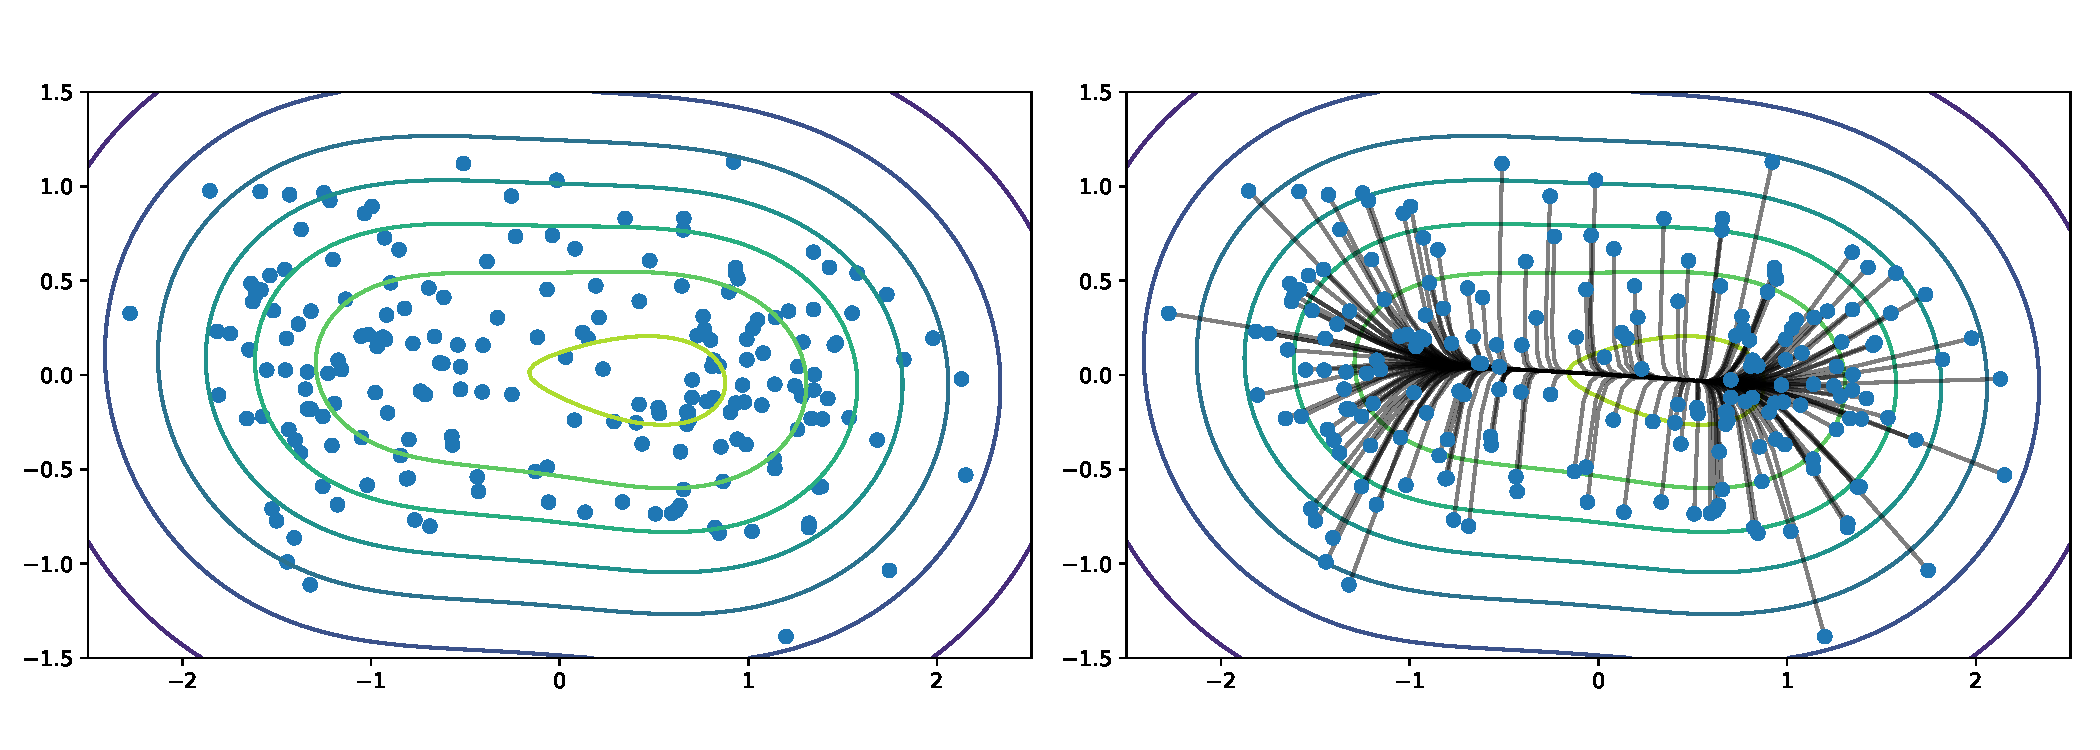
\includegraphics[height=0.4\textheight]{{{figures/contour/kde-and-trajectories-h=0.8-K=gaussian}}} \\[-2mm]
		$h=0.8$, gaussian kernel \\
		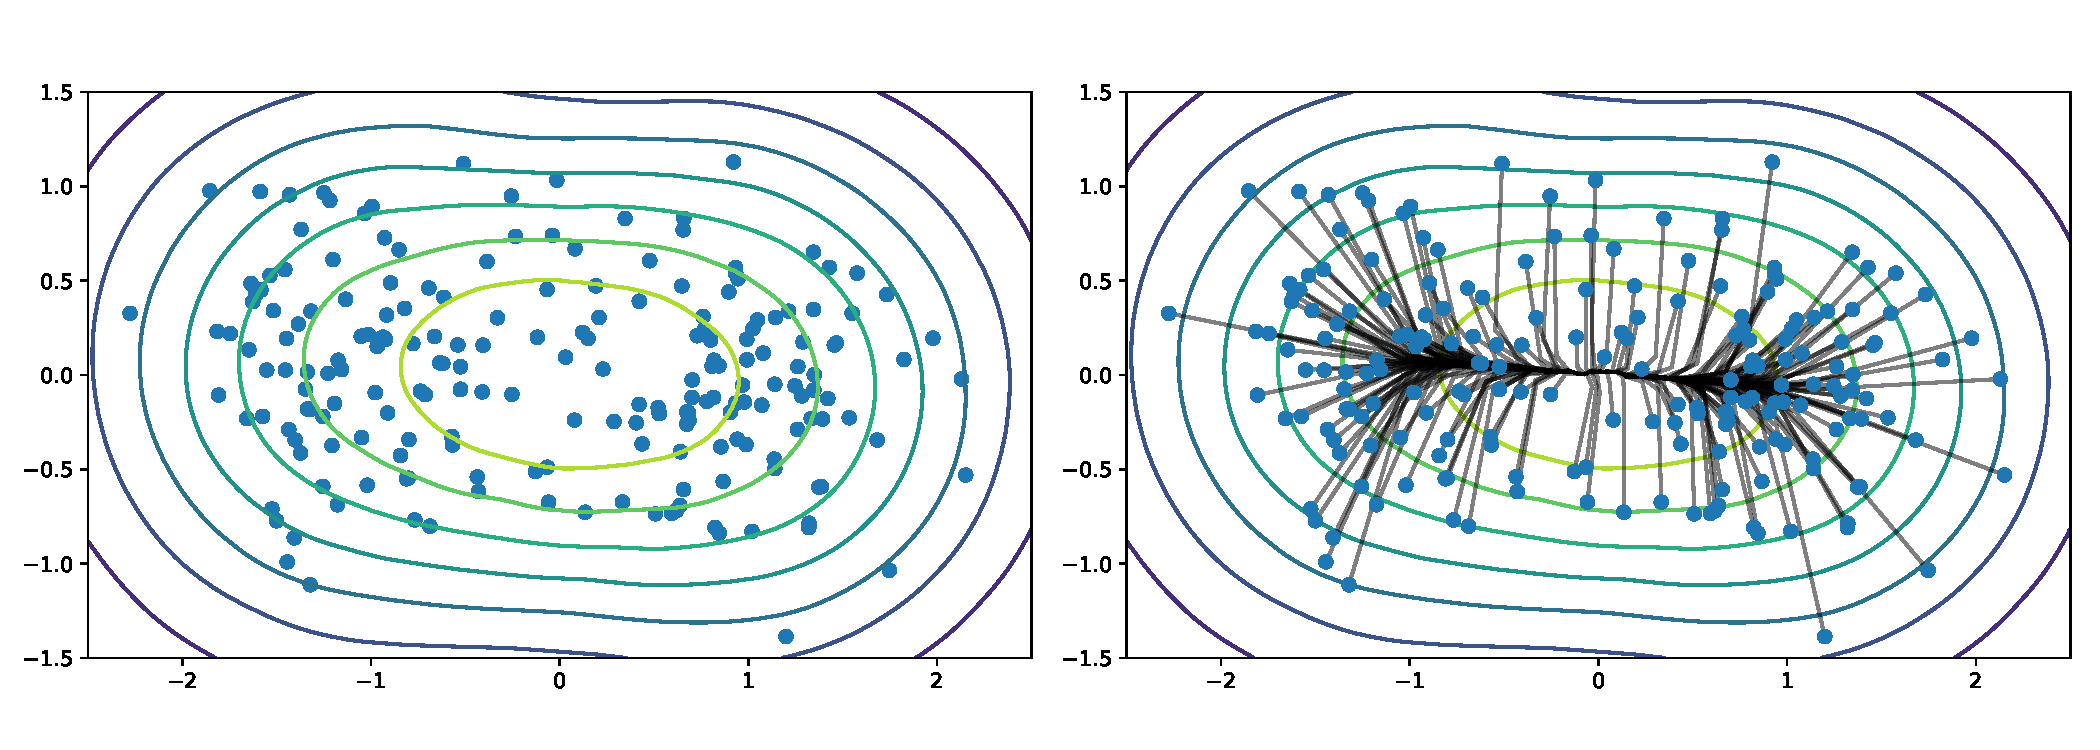
\includegraphics[height=0.4\textheight]{{{figures/contour/kde-and-trajectories-h=1.7-K=uniform}}} \\[-2mm]
		$h=1.7$, uniform kernel
	\end{tabular}
\end{figure}
\end{frame}


\begin{frame}<0>{Advantages}
% TODO: from text
\begin{itemize}
	\item One of the main benefits is that the algorithm makes no prior assumptions about the number and shape of the clusters. This allows complex clusters with non-convex shapes.
	
	\item Outliers do not affect the clustering of the other data points. As outliers lie in low density regions their weight assigned by the kernel is either zero or very small.
	
	\item The algorithm only has one parameter, the bandwidth. The bandwidth has a easily understood interpretation and determines the resulting cluster uniquely. That can be used to formulate functions dependent on the bandwidth, e.g. some clustering criteria.
	
	\item The cluster centroids can be interpreted as the modes of the estimated density function. That has the benefit that, ignoring the outliers, the centroids are ``typical'' data objects in that they are from a locally high-density environment.
\end{itemize}
\end{frame}

\begin{frame}<0>{Disadvantages}
% TODO: from text
\begin{itemize}
	\item The algorithm has complexity $\mathcal{O}(Tn^2)$, with $T$ being the number of iterations. This is especially problematic for large datasets.
	
	\item A problem originating from the underlying multivariate kernel density estimation is a poor scaling with the dimension of the feature space $d$.
	
	\item As we have already discussed in section \ref{sec:bandwidth-selection}, it is not easy to find a fitting bandwidth, especially in the multivariate case.
	
	\item Although the modes are local maxima, it is not guaranteed that they lie in a large density environment. This can easily be fixed by a post processing step in which low density modes are classified as outliers.
	
	\item In some use cases it is useful to specify the number of clusters a priori. This is only possible by searching for the desired number of clusters through changing the bandwidth.
\end{itemize}
\end{frame}

\begin{frame}{Discussion}
	\textbf{Advantages}
	\begin{itemize}
		\item No prior assumption on cluster shapes. Complex and non-convex shapes are possible
		\item Only has one tuning parameter, the bandwidth
		\item No restriction on number of clusters
		%\item Cluster centroids are local maxima of the density
		\item Outliers do not affect the clustering
	\end{itemize}
	\textbf{Disadvantages}
	\begin{itemize}
		\item Density estimation fails for high dimensions ($\approx d$ > 5)
		\item Bad computational complexity $\mathcal{O}(Tn^2)$
		\item Finding a good bandwidth is hard
	\end{itemize}
\end{frame}

\begin{frame}<0>{Pros and Cons}
% TODO: copied from other source
	\textbf{Pros}
	\begin{itemize}
		\item Does not assume spherical clusters
		\item Just a single parameter (window size)
		\item Finds variable number of modes
		\item Robust to outliers
	\end{itemize}
	\textbf{Cons}
	\begin{itemize}
		\item Output depends on window size
		\item Computationally expensive
		\item Does not scale well with dimension of feature space
	\end{itemize}
\end{frame}


\section{Application}

\begin{frame}{Application -- Image segmentation}
\begin{figure}	
	\begin{tabular}{cc}
		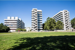
\includegraphics[height=0.4\textheight]{{{figures/kit-demo/image-resized}}} &
		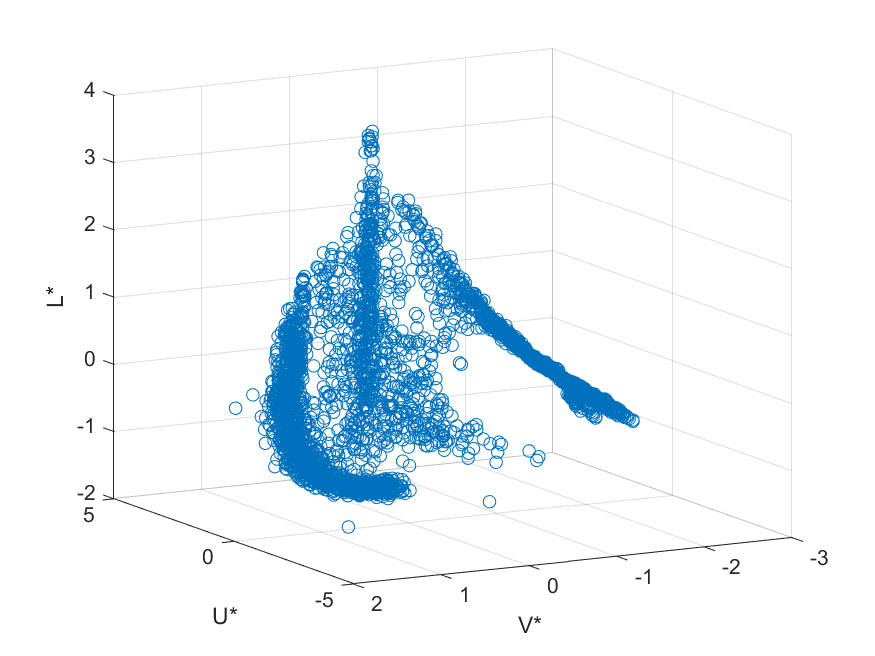
\includegraphics[height=0.5\textheight]{{{figures/kit-demo/scatter-plot}}}
	\end{tabular}
\end{figure}
\begin{itemize}
	\item Image data can be represented as data points. The pixels can be clustered and the clustering results in a segmentation of the original image.
\end{itemize}
\end{frame}


\begin{frame}{Image segmentation -- Gaussian kernel}
\tiny
\begin{figure}
	\begin{tabular}{cc}
		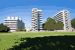
\includegraphics[height=0.3\textheight]{{figures/kit-demo/image-segmentation-h=0.1-K=gaussian}.png} &   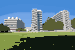
\includegraphics[height=0.3\textheight]{{figures/kit-demo/image-segmentation-h=0.2-K=gaussian}.png} \\
		(a) $h = 0.1$ & (b) $h = 0.2$ \\[6pt]
		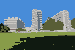
\includegraphics[height=0.3\textheight]{{figures/kit-demo/image-segmentation-h=0.3-K=gaussian}.png} &   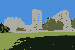
\includegraphics[height=0.3\textheight]{{figures/kit-demo/image-segmentation-h=0.4-K=gaussian}.png} \\
		(c) $h = 0.3$ & (d) $h = 0.4$ \\[6pt]
	\end{tabular}
\end{figure}
\end{frame}


\begin{frame}{Image segmentation -- Gaussian kernel}
\tiny
\begin{figure}
\begin{tabular}{cc}
	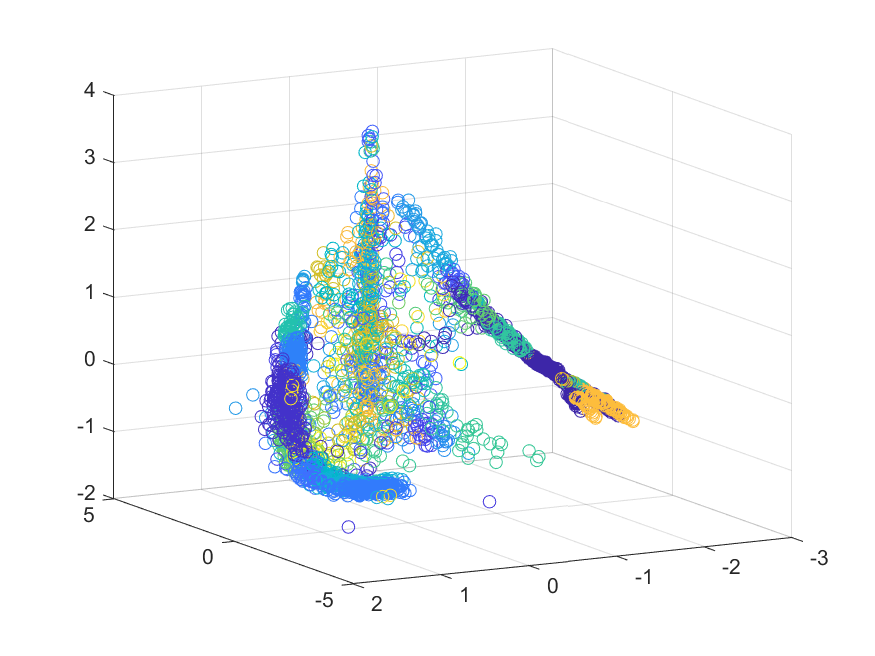
\includegraphics[height=0.3\textheight]{{figures/kit-demo/scatter-plot-h=0.1-K=gaussian}.png} &   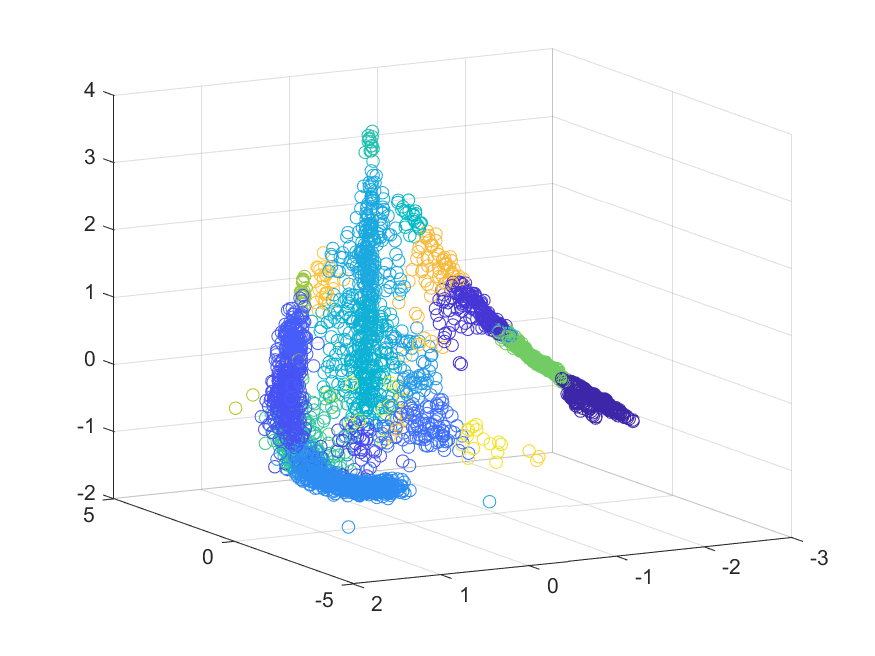
\includegraphics[height=0.3\textheight]{{figures/kit-demo/scatter-plot-h=0.2-K=gaussian}.png} \\
	(a) $h = 0.1$ & (b) $h = 0.2$ \\[6pt]
	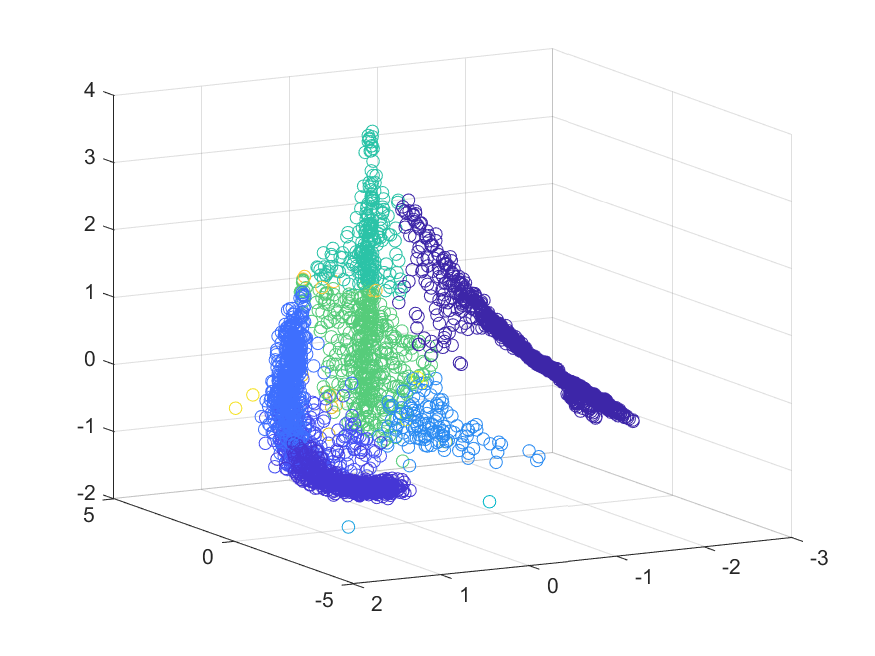
\includegraphics[height=0.3\textheight]{{figures/kit-demo/scatter-plot-h=0.3-K=gaussian}.png} &   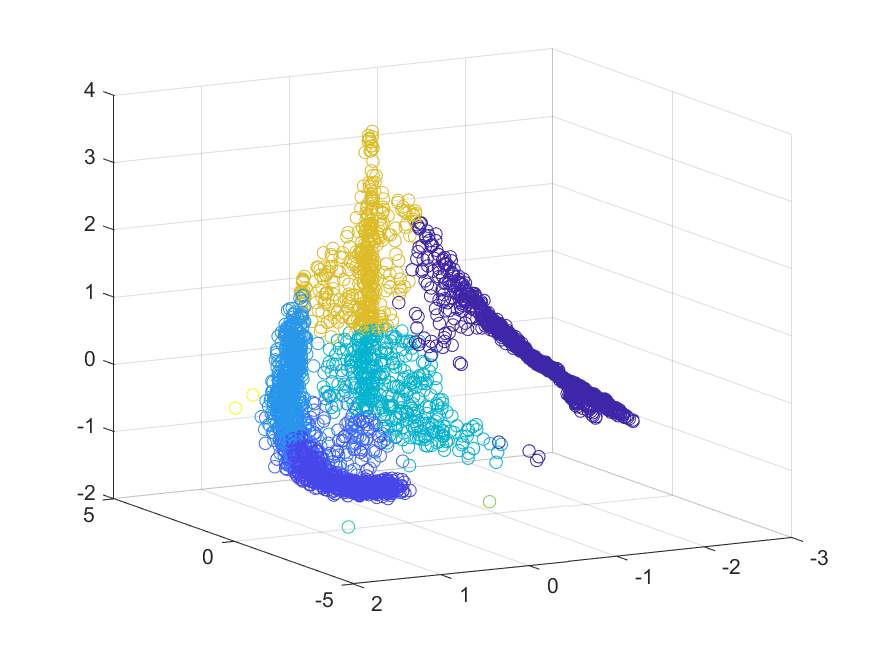
\includegraphics[height=0.3\textheight]{{figures/kit-demo/scatter-plot-h=0.4-K=gaussian}.png} \\
	(c) $h = 0.3$ & (d) $h = 0.4$ \\[6pt]
\end{tabular}
\caption{caption}
\end{figure}
\end{frame}


\begin{frame}{Image segmentation -- Uniform kernel}
\tiny
\begin{figure}
\begin{tabular}{cc}
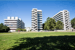
\includegraphics[height=0.3\textheight]{{figures/kit-demo/image-segmentation-h=0.1-K=uniform}.png} &   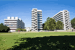
\includegraphics[height=0.3\textheight]{{figures/kit-demo/image-segmentation-h=0.2-K=uniform}.png} \\
(a) $h = 0.1$ & (b) $h = 0.2$ \\[6pt]
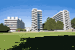
\includegraphics[height=0.3\textheight]{{figures/kit-demo/image-segmentation-h=0.3-K=uniform}.png} &   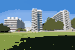
\includegraphics[height=0.3\textheight]{{figures/kit-demo/image-segmentation-h=0.4-K=uniform}.png} \\
(c) $h = 0.3$ & (d) $h = 0.4$ \\[6pt]
\end{tabular}
\end{figure}
\end{frame}


\begin{frame}{Image segmentation -- Uniform kernel}
\tiny
\begin{figure}
\begin{tabular}{cc}
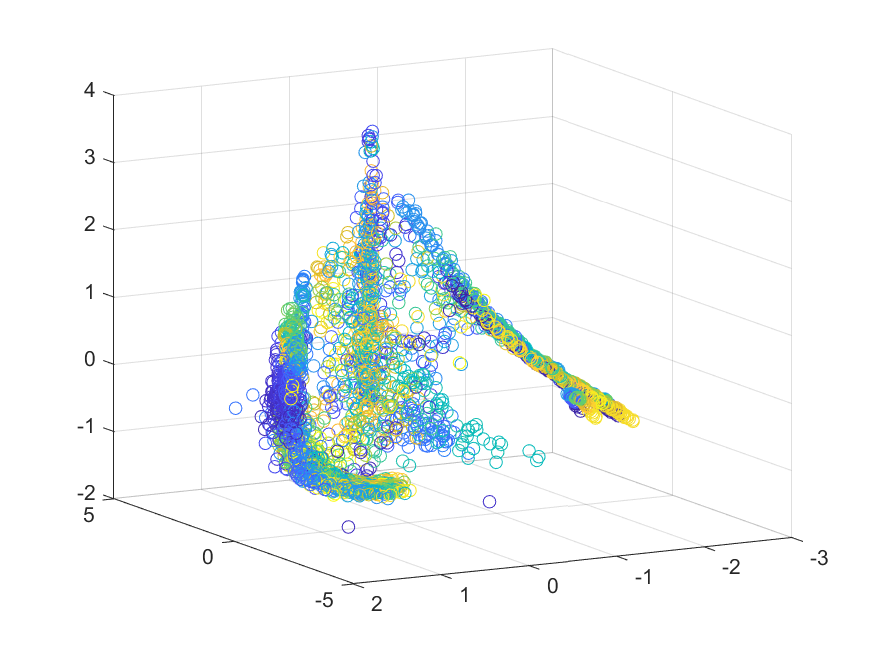
\includegraphics[height=0.3\textheight]{{figures/kit-demo/scatter-plot-h=0.1-K=uniform}.png} &   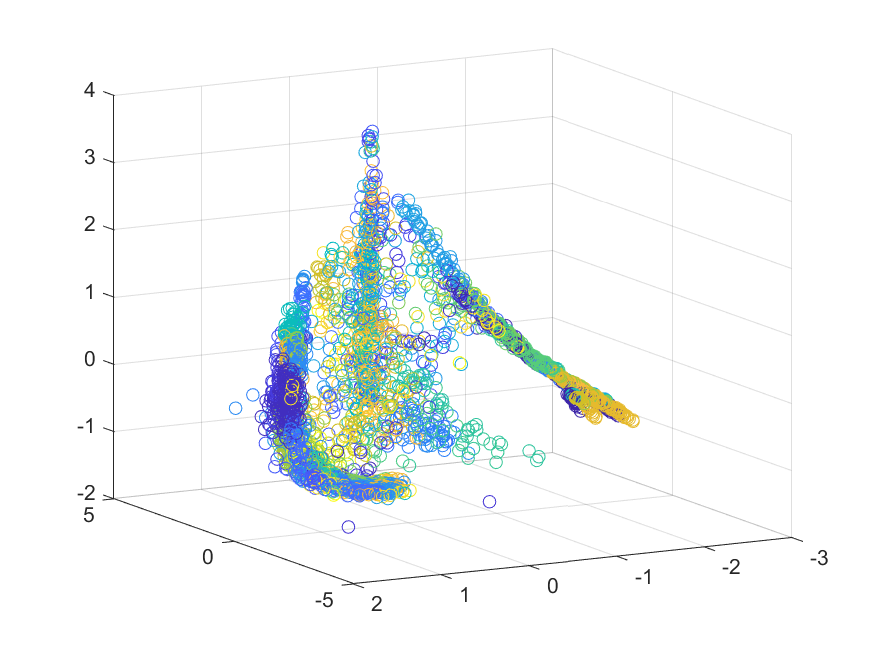
\includegraphics[height=0.3\textheight]{{figures/kit-demo/scatter-plot-h=0.2-K=uniform}.png} \\
(a) $h = 0.1$ & (b) $h = 0.2$ \\[6pt]
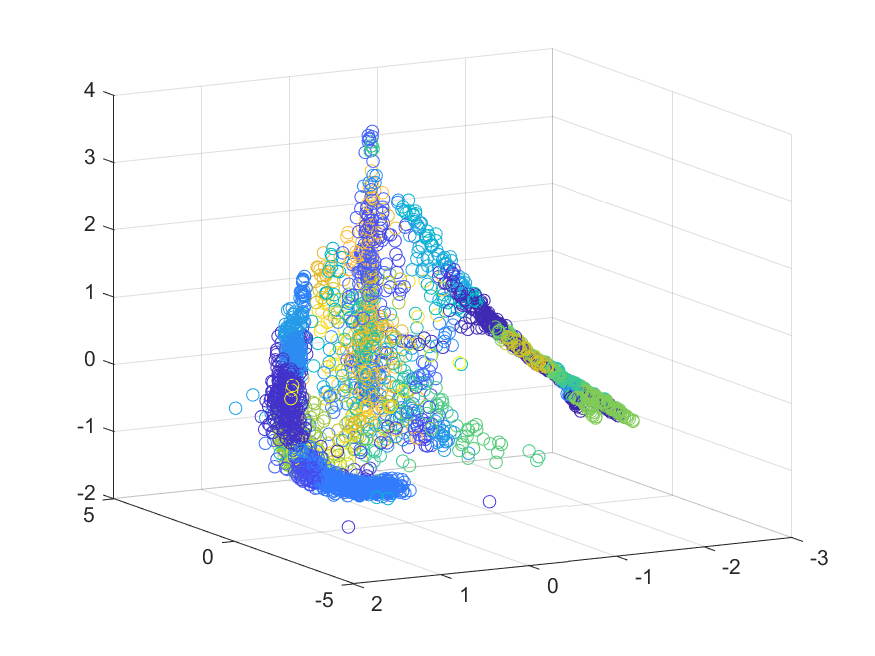
\includegraphics[height=0.3\textheight]{{figures/kit-demo/scatter-plot-h=0.3-K=uniform}.png} &   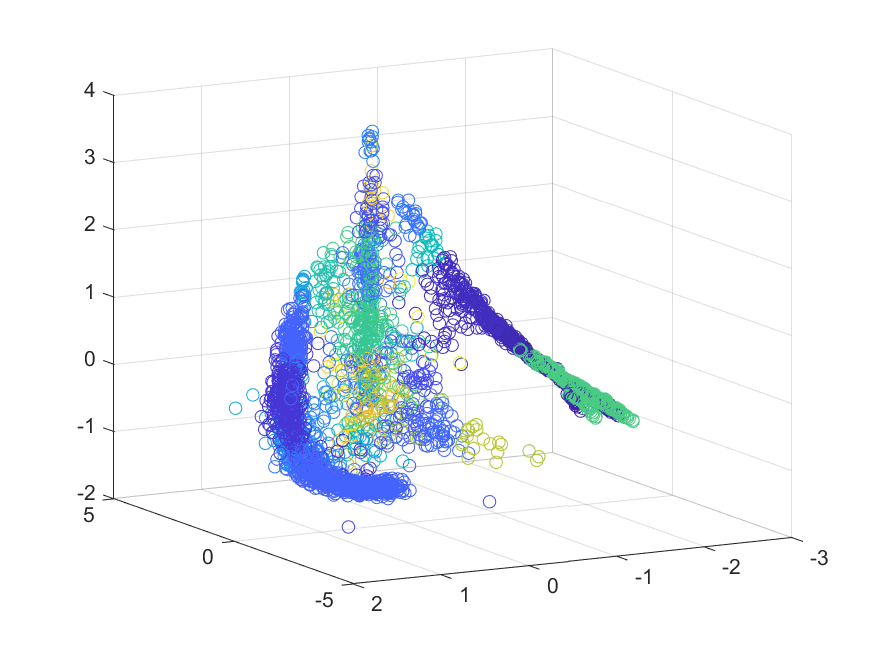
\includegraphics[height=0.3\textheight]{{figures/kit-demo/scatter-plot-h=0.4-K=uniform}.png} \\
(c) $h = 0.3$ & (d) $h = 0.4$ \\[6pt]
\end{tabular}
\end{figure}
\end{frame}



%\section{Suchen und Sortieren}
%\subsection{Insertionsort}
%\begin{frame}
%\begin{algorithm}[H]
%	\caption{Euclid’s algorithm}\label{euclid}
%	\begin{algorithmic}[1]
%		\Procedure{Euclid}{$a,b$}\Comment{The g.c.d. of a and b}
%		\State $r\gets a\bmod b$
%		\While{$r\not=0$}\Comment{We have the answer if r is 0}
%		\State $a\gets b$
%		\State $b\gets r$
%		\State $r\gets a\bmod b$
%		\EndWhile\label{euclidendwhile}
%		\State \textbf{return} $b$\Comment{The gcd is b}
%		\EndProcedure
%	\end{algorithmic}
%\end{algorithm}
%\end{frame}


\appendix
\beginbackup

\begin{frame}[allowframebreaks]{References}
	%\printbibliography
	
	\bibliographystyle{agsm}
	\bibliography{../latex/KDEaMSC}
\end{frame}

\begin{frame}
	\listoffigures
\end{frame}

\backupend

\end{document}
